\documentclass{article}
\usepackage[margin=1in]{geometry}
\usepackage{multicol}
\usepackage{blindtext}
\usepackage{graphicx}
\usepackage{pgfplots}
\usepackage{pgfplotstable}
\usepackage{tikz}
\usetikzlibrary{shapes.geometric, arrows}

\definecolor{testorange}{HTML}{FFAD7A}
\definecolor{clear}{HTML}{E3E9FD}
\definecolor{magenta}{HTML}{C60059}
\definecolor{yellow}{HTML}{F0C500}
\definecolor{cyan}{HTML}{0089A6}
\definecolor{targetblue}{HTML}{1a4d66}

\usepackage{draftwatermark}
\SetWatermarkText{DRAFT. NOT REVIEWED OR COMPLETED}
\SetWatermarkScale{1}

\title{Polyjet Voxel Printing Exploration}

\author{Jack Crane}
\date{\today}

\begin{document}

\noindent
\LARGE\textsl{Printing complex geometry with complex materials}
\vspace*{-.3cm} 

\noindent
\Huge Polyjet Voxel Printing Exploration 
\vspace*{.25cm} 

\noindent
\large Jack Crane \textit{jack.crane@slu.edu}

\noindent
\large Saint Louis University Center for Addditive Manufacturing \textit{slu.cam@slu.edu}
\normalsize
\\\\
\noindent\fbox{%
    \parbox{\textwidth}{%
        \textit{Notice:} Content, algorithms, logic, and references in this document are not peer-reviewed, verified, authorized, and should not be interpreted as an authority. Content contained herein may be hypothetical or experimental, and should be evaluated critically by the reader. Any application or use of the information provided is at the sole risk and discretion of the user. The creators of this document bear no responsibility for any consequences arising from the use of the information contained within. This document is not intended for public consumption at this time and until published, all content should be considered confidential.
    }%
}
\\

%\begin{multicols}{2}
\tableofcontents
%\end{multicols}

\vspace*{\fill}
\noindent
\hspace*{-.3cm}   
\includegraphics[width=.25\columnwidth]{slucam-logo}

\noindent
\includegraphics[width=.2\columnwidth]{slu}

\pagebreak

\begin{multicols}{2}
\section{Introduction \& Background}
I wanted to be able to print random objects that could be mathematically defined and 3d printed on our PolyJet 3d printing system. Once parts become complex, colorful, or more unique, it is necessary to begin using customized slicers for more advanced solutions. My first objective is to replicate a part that SLUCAM had when I was looking at schools. It was several inches long, about an inch wide, about $\frac{1}{10}$ of an inch thick. It featured a gradient from white to a color, and from flexible to hard as it went along, the white as flexible and the color as hard. After some discussion, it was made clear that the only way to achieve this is to write some code that would generate the voxel cloud that we could then parse into a print job. The GrabCAD voxel printing documentation\footnote{https://help.grabcad.com/article/230-guide-to-voxel-printing?locale=en} served as a good place to start, providing background on the printer setup, such as resolution, layer height, colors, and formats. 

\subsection{Colors} From Michael and the documentation, I have learned that the printer cannot extrapolate the colors to use from merely an imported image, the image must already be split into colors. The Voxel Print Utility expects a small number of colors to be present in the provided PNG sequence, and assumes materials to use based on colors provided. Color assumptions are made based on this table excerpt:
\\\\
\noindent
\begin{tabular}{|c||c|c|c||c|}
    \hline
    Base Resin & Red & Green & Blue & Hex \\
    \hline
    Agilus30Wht & 255 & 255 & 255 & \#FFFFFF \\
    VeroClear & 227 & 233 & 253 & \#E3E9FD \\
    VeroMGT-V & 198 & 0 & 88 & \#C60058 \\
    VeroYL-V & 240 & 197 & 0 & \#F0C500 \\
    VeroCY-V & 0 & 137 & 166 & \#0089A6 \\
    (Void) & 0 & 0 & 0 & \#000000 \\
    \hline
\end{tabular}
\\\\\\
\noindent
This table comes from the GrabCAD Voxel Printing Documentation. I have removed information on resins we do not have loaded in our machine for brevity. How we have the printer configured, the slicer expects these (and only these colors) be supplied. While these specific colors are not \textit{required} as colors can be re-mapped from inside the Voxel Print utility, using the assigned colors helps the utility to automatically assume resins without manual configuration. 

\subsection{Resolution \& DPI}
The printer is configured strangely in how it handles resolution. The Voxel Print documentation calls out that a 600 x 300 pixel image will serve as a 1 inch square, and a 600 x 600 pixel image will draw a rectangle. I found it hard to understand this configuration, but a 600 x 600 pixel print will print oriented as such:
\\\\
\includegraphics[width=0.5\textwidth]{600x600-print-orientation}

\noindent
Beware while designing that once you prepare your PNG layers, you cannot change their orientation in the software. You are able to translate, but cannot rotate your print, so the software must be written to take this into account while slicing. 

\section{System Design}

This is not SLUCAM's first exploration into learning and perfecting the use of the voxel printing methods. Past explorations used Matlab to create the contents, but I chose to use JavaScript in my explorations due to my relative comfort in JavaScript and out of wanting to define methods in another language.

\subsection{File \& Organization}
The voxel print utility expects a folder of PNG files, each with the same dimensions and color schema. The files must be consistently named using a prefix convention and each PNG is a layer. My prints use a `slice\_\{layer number\}.png' naming scheme, but any file names using a consistent prefix and a sequential value symbolizing the layer height.
\\\\
\noindent
\includegraphics[width=0.5\textwidth]{string-padding}
\\

\noindent
For ease of management, the files live in an output folder that can be zipped and transferred elsewhere or directed into GrabCAD Print Voxel Print Utility directly. 

\subsection{Language Choice}

For this project I elected to use JavaScript to implement these features. Unlike previous work done in SLUCAM I opted to use JavaScript over Matlab. Previous work has been done in Matlab because it is a powerful math/vector language. I opted to use JavaScript because of familiarity and it's relative efficiency thanks to its ability to use the GPU to write image files. (which may be put to the test). Although cross-platform support is not something we care about now, the flexibility and universality of JavaScript made it alluring because of the option to deploy this work to other devices and platforms. Because JavaScript is freely available and non-proprietary, a potential user does not need to have Matlab installed and own a license.

\subsection{Performance}

While JavaScript may not be the most performant language, especially when dealing with large amounts of data or vectors, it is still able to hold its own against most languages and has nice benefits when datasets become large. Figures 2.3.1-2 highlight how the performance changes across layers. Figure 2.3.1 shows how performance worsens more-or-less linearly with the size of the image. These performance graphs have not been overly systematically generated, but are accurate enough to provide an approximate understanding of how performance will change. Performance was measured on a 2022 M2 MacBook Air with 8gb of memory.

\

\subsubsection{Performance on a 600x600 image}

\pgfplotstableread{
Trial  Random  Draw  Export
{Slice 0}   15    136    37
{Slice 25}   14     135    37
{Slice 50}  14		136		42
{Slice 99}	14	140	38
}\sixhundred

\noindent
\resizebox{\columnwidth}{!}{

\begin{tikzpicture}

\begin{axis}[
        ybar stacked,
        bar width=30pt,
        height=6cm,
        width={\columnwidth},
        ylabel={Execution Time (ms)},
        xtick=data,
        xticklabels from table={\sixhundred}{Trial},
        legend style={
            at={(0.5,1.12)},
            anchor=north,
            legend columns=-1,
            font=\tiny
        },
        nodes near coords,
        every node near coord/.append style={font=\tiny, anchor=north, text=black}
        ]
        \addplot+[ybar] table [x expr=\coordindex, y=Random] {\sixhundred};
        \addplot+[ybar] table [x expr=\coordindex, y=Draw] {\sixhundred};
        \addplot+[ybar] table [x expr=\coordindex, y=Export] {\sixhundred};
        
        \legend{Random fill, Compute \& Draw, Render \& File Write}
    \end{axis}

\end{tikzpicture}

}

\subsubsection{Performance on a 1200x600 image}

\pgfplotstableread{
Trial  Random  Draw  Export
{Slice 0}   32 266 73
{Slice 25}   29 271 73
{Slice 50}  27 266 73
{Slice 99}	27 269 73
{Ref.}	14	140	38
}\twelvehundred

\noindent
\resizebox{\columnwidth}{!}{

\begin{tikzpicture}

\begin{axis}[
        ybar stacked,
        height=6cm,
        width={\columnwidth},
        bar width=30pt,
        ylabel={Execution time (ms)},
        xtick=data,
        xticklabels from table={\twelvehundred}{Trial},
        legend style={
            at={(0.5,1.12)},
            anchor=north,
            legend columns=-1,
            font=\tiny
        },
        nodes near coords,
        every node near coord/.append style={font=\tiny, anchor=north, text=black}
        ]
        \addplot+[ybar] table [x expr=\coordindex, y=Random] {\twelvehundred};
        \addplot+[ybar] table [x expr=\coordindex, y=Draw] {\twelvehundred};
        \addplot+[ybar] table [x expr=\coordindex, y=Export] {\twelvehundred};
        
        \legend{Random fill, Compute \& Draw, Render \& File Write}
    \end{axis}

\end{tikzpicture}

}

\noindent
\textit{The ``Ref." entry is Slice 99 from the 600x600 image provided for comparison.}

\subsubsection{Performance on $n$-sized images}


\pgfplotstableread{
Trial  Random  Draw  Export
{6x6}   15 136 37
{6x12}   27 266 73
{6x18}  42 403 107
{6x24}	61 536 146
{6x30} 75 682 187
}\scaledata

\begin{tikzpicture}
\begin{axis}[
    xlabel={Image Size (*100)},
    ylabel={Execution time (ms)},
    legend pos=north west,
    ymajorgrids=true,
    xtick=data,
    xticklabels from table={\scaledata}{Trial},
    width={\columnwidth}
]
\addplot table[x expr=\coordindex,y=Random]{\scaledata};
\addlegendentry{Random}
\addplot table[x expr=\coordindex,y=Draw]{\scaledata};
\addlegendentry{Draw}
\addplot table[x expr=\coordindex,y=Export]{\scaledata};
\addlegendentry{Export}
\end{axis}
\end{tikzpicture}

\section{Strategy \& Algorithms}
There are a few sub-algorithms that need designed and strategized to make sure the part can be generated. There were several strategies considered including a ``cascading-cell" pixel fill algorithm that would generate recurring, consistent $n\times n$ cells that would hold a predictable pattern of colored voxels, and a ``random-fill" algorithm that fills a helper array with random values then uses a loop's progress to determine the color to display on a per-pixel base. I decided to go with the random-fill algorithm because of it's relative simplicity and it's basis seeming simpler and more flexible.

\subsection{Gradient Generation} \label{gradient generation}

\subsubsection{Linear Gradient Generation}
A linear gradient is the simplest and most bare-bones approach to generating a gradient and is the first strategy I chased. The algorithm worked by creating a ``ghost" array that is filled with random numbers uniformly distributed between 0 and 1 (represented as the large non-italicized numbers in the number grid). Then as the loop iterates through the ``rows" of the array, it computes it's progress by $row_{current}/row_{total}$, where $row_{total}$ comes from the resolution configuration. This is the small italicized numbers in the grid. Finally, it compares the progress to the random, and if the progress is larger, the pixel gets filled.
\\

\noindent
\includegraphics[width=\columnwidth]{slice_000_rand}
\\

\noindent
Each square represents a pixel of this 6x3 example. The first pixel (top left) has a random value of 0.09, and a progress value of 0.00. Because 0.09 is greater than 0.00, that pixel does not get colored and is set to the color denoting Agilus 30 White, \#FFFFFF. Now looking at the bottom left pixel, it has a random value of 0.24 and a progress value of 0.67. Because the progress value is greater than the random number, the pixel gets filled.
\\

\noindent
\includegraphics[width=\columnwidth]{slice_000_scaled}
\\

\noindent
Once the algorithm is defined, the resolution can just be increased and the gradient pixel fill will scale.

\

\noindent
\includegraphics[width=\columnwidth]{slice_000}
\\

\noindent
However, this highlights a multitude of issues based in color theory and the corrections that need to be applied to force colors to show as intended. This above gradient looks \textit{perfect}. It features a smooth, linear transition from blue to white. However, colors and materials do not mesh like this in the real world, as when this gradient was printed, we were met with this\footnote{This print was generated with the same algorithm as the gradient image, but was printed at a 600x600, not 600x300 resolution like the large-resolution image above.}:
\\

\noindent
\includegraphics[width=.505\columnwidth]{linear-gradient-print}
\includegraphics[width=.485\columnwidth]{linear-gradient-print-light}
\\

\noindent
A distinctly \textit{nonlinear} gradient from blue to white. This helps illustrate how the darker blue color overpowers the more gentle white. Color implementations are also affected by the specific materials loaded in our printer, in this case Agilus 30 White and Vero Cyan Vivid. As highlighted by the picture holding the print up to the light, Vero Cyan is slightly transparent and when not backed by white is an extremely dark blue. This is typically solved digitally using a technique called ICC Color Correction to help translate between different color spaces. However, we are not able to use existing color correction techniques without thought and modification because existing color correction techniques are either based on the RGB (or RGB based) color space, or the CMYK color space. Neither of these apply as they are because RGB is \textit{emissive}, and CMY(+K) assume they are being laid on a bright and somewhat reflective white surface. When Polyjet 3d printing, we have neither to work with. The approach we will have to hone in on will be based on the CMY(+W) architecture because those are the colors that are available in our printer.
\\
This gradient may also be pushed into a nonlinear space because the more powerful dark blue is transparent and there are subsurface layers that have blue material in overlapping positions and the random pixel fill algorithm generates a randomly seeded gradient on each layer. I Also wanted to experiment with using a consistent random gradient for each layer, where the position of the blue and white voxels would be either the same on each layer (bottom), or randomly shuffled for each layer (top).  This resulted in a distinctly different appearance, durometer, and flexibility.

\noindent
\includegraphics[width=\columnwidth]{grainy-vs-not-gradient}

\noindent
Somewhat unsurprisingly, the part made without the random dispersion was extremely grainy, driven from the fact that there is no offset provided by the colors behind. Interestingly, with eyes closed, their flexibility is nearly indistinguishable.

\subsubsection{Nonlinear B\'ezier-driven Gradient}

In my first approach to creating a nonlinear approach to creating a smooth gradient, I decided to take a ``stop layer" between a straight linear gradient and a mathematically, color-theory-heavy approach, I wanted to experiment and tweak the gradient generation between print jobs. There are several approaches to this kind of experimentation-friendly program, but I chose to create an implementation of a standard 2-node b\'ezier curve.
\\

\noindent
\begin{tabular}{|p{.23\columnwidth}||p{.2\columnwidth}|p{.2\columnwidth}|p{.15\columnwidth}|}
    \hline
    B\'ezier point & Material & Attribute & Default \\
    \hline
    $p_0$ & Color & Falloff & 0  \\
    $p_1$ & Color & Basis & 0  \\
    $p_2$ & White & Falloff & 1  \\
    $p_3$ & White & Basis & 1  \\
    \hline
\end{tabular}

\noindent
\includegraphics[width=.5\columnwidth]{0011}
\includegraphics[width=.5\columnwidth]{0515}
\includegraphics[width=.5\columnwidth]{5515}
\includegraphics[width=.5\columnwidth]{0555}

\noindent
These images are examples of the gradient will react to different curve configurations. These images are based on b\'ezier attributes of \textit{(0,0,1,1)}, \textit{(0,5,1,5)}, \textit{(5,5,1,5)}, and \textit{(0,5,5,5)} respectively. The ``vertical" position of each handle (corresponding to $p_1$ and $p_3$) controls the \textit{basis}, or the overall strength of the color. Functionally, this tends to influence where the solid-color part of the gradient ends and the transition begins. The ``horizontal" component controls the \textit{falloff} of the color, or how aggressively it transitions into the gradient color.

\section{Generating more colors}

The printer only has the cyan, magenta, yellow, and white resins installed, so if we wanted to print something that is not one of the pre-installed colors (say, \fcolorbox{black}{testorange}{\rule{0pt}{6pt}\rule{6pt}{0pt}} \#FFAD7A), we need to merge voxels of other colors in ratios that will end up producing the ``end goal" color. There are a few steps to getting to these ratios. The result of my initial exploration into generating a part with that color resulted in a partial success.
\\

\noindent
\includegraphics[width=\columnwidth]{ffad7a-result-1}

\subsection{Converting to HSV} \label{converting to hsv}

The HSV color space provides the algorithm more context on the objective color because it gives us a hue, which serves as a color attribute without lightness or saturation having come into play, saturation, which serves as a ratio of how much color vs an illumination ratio, and the value, which serves as said illumination ratio. For the sake of explanation, consider the objective color as \fcolorbox{black}{targetblue}{\rule{0pt}{6pt}\rule{6pt}{0pt}} \#1a4d66. The first step is to convert the hexadecimal value into an RGB color, resulting in [26, 77, 102]. The next step is to convert the RGB values into HSV components. I used existing color conversion logic, but the conversion from RGB to HSV is neither complex no novel, so will not be covered in further detail. The output from the HSV conversion turns out to be [$200^\circ$, 75\%, 40\%]. In practice, the HSV implementation in a physical ratio format is as depicted below. The first component (the hue) is the position on the outer rim of the color wheel that the objective color falls, or in this case, 200 degrees counter-clockwise from the 12 o'clock position. The saturation, or how strong the color is serves as the ratio of the colored portion to the colorless portion, in this case 75\%, meaning that 3/4 voxels should be dedicated to reaching the desired color, and 1/4 is dedicated to the value component. The value, or amount of darkness in the color, is the percentage of ``black" to white in the mix, or in this case 40\%. In our real slices, these all should be mixed up, but for the sake of demonstration, this graphic shows the relative amount of each color group.

\noindent
\tikzset{every picture/.style={line width=0.75pt}} %set default line width to 0.75pt        

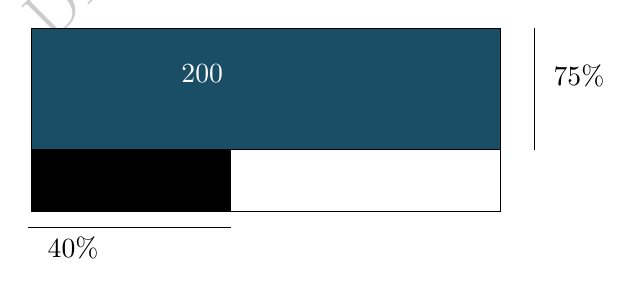
\begin{tikzpicture}[x=0.75pt,y=0.75pt,yscale=-1.5,xscale=3.25]
\draw  [fill={rgb, 255:red, 26; green, 77; blue, 102 }  ,fill opacity=1 ] (0.5,1) -- (70,1) -- (70,40) -- (0.5,40) -- cycle ;
\draw   (0.5,40) -- (70,40) -- (70,60) -- (0.5,60) -- cycle ;
\draw    (75,1) -- (75,40) ;
\draw  [fill={rgb, 255:red, 0; green, 0; blue, 0 }  ,fill opacity=1 ] (0.5,40) -- (30,40) -- (30,60) -- (0.5,60) -- cycle ;
\draw    (0,65) -- (30,65) ;

% Text Node
\draw (77.5,12) node [anchor=north west][inner sep=0.75pt]   [align=left] {75\%};
% Text Node
\draw (22.33,12) node [anchor=north west][inner sep=0.75pt]  [color={white}  ,opacity=1 ] [align=left] {200};
% Text Node
\draw (2.5,67) node [anchor=north west][inner sep=0.75pt]   [align=left] {40\%};


\end{tikzpicture}

\noindent
Using the same logic as we used to distribute colors randomly in the gradient, we can go about distributing pixels. This is done by creating the randomly seeded random value array, and (in this case), if that random number is below 0.75, assign the blue color. Otherwise, we go into a nested random checker where a new random number is generated for that pixel. If the random number is below 0.4, the pixel gets assigned black, and otherwise, the pixel is assigned white. The image on the left is an example of the output generated by this algorithm.
\\


\noindent
\includegraphics[width=\columnwidth]{objective-color-hsv-no-color-seperation}
\\

\noindent
This works great except it doesn't actually solve our problem all the way. It is able to normalize the color so that the lightness\footnote{Not to be confused with the lightness component of an HSL color. We are using HSV, not HSL, and while they are similar, it is important to note that anytime lightness or darkness is referenced in this paper, it is in reference to the value component.} or contrast of the color is not a factor and allows it to be more granually controlled in the part, but it still uses the blue color which is not installed, and still uses black to describe darkness, which is likewise not installed. 

\subsection{Converting from hue to CMY}

To convert from hue (the first component returned from the HSV conversion) to CMY, it is important to understand the color wheel. This extremely simple rendition of the color wheel highlights the positions of yellow, magenta, and cyan, the degree positions of each, the degree travels between each color, and the position of our color of focus at the $200^\circ$ position. 
\\

\tikzset{every picture/.style={line width=0.75pt}} %set default line width to 0.75pt        

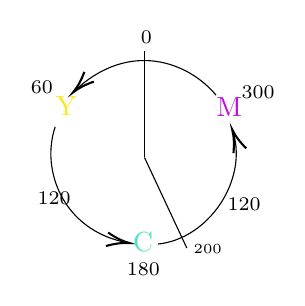
\begin{tikzpicture}[x=0.75pt,y=0.75pt,yscale=-1,xscale=1]
%uncomment if require: \path (0,300); %set diagram left start at 0, and has height of 300

%Curve Lines [id:da04176240931286035] 
\draw [color={rgb, 255:red, 0; green, 0; blue, 0 }  ,draw opacity=1 ]   (14.25,49.92) .. controls (7.14,70.74) and (18.05,99.49) .. (48.13,105.57) ;
\draw [shift={(50,105.92)}, rotate = 189.46] [color={rgb, 255:red, 0; green, 0; blue, 0 }  ,draw opacity=1 ][line width=0.75]    (10.93,-3.29) .. controls (6.95,-1.4) and (3.31,-0.3) .. (0,0) .. controls (3.31,0.3) and (6.95,1.4) .. (10.93,3.29)   ;
%Curve Lines [id:da7326294363276744] 
\draw    (63.75,106.42) .. controls (88.61,103.74) and (106.82,75.39) .. (100.07,52.89) ;
\draw [shift={(99.5,51.17)}, rotate = 70.07] [color={rgb, 255:red, 0; green, 0; blue, 0 }  ][line width=0.75]    (10.93,-3.29) .. controls (6.95,-1.4) and (3.31,-0.3) .. (0,0) .. controls (3.31,0.3) and (6.95,1.4) .. (10.93,3.29)   ;
%Curve Lines [id:da8437766801809956] 
\draw    (91.75,34.67) .. controls (78.45,18.66) and (50.12,7.99) .. (23.94,32.28) ;
\draw [shift={(22.75,33.42)}, rotate = 315.82] [color={rgb, 255:red, 0; green, 0; blue, 0 }  ][line width=0.75]    (10.93,-3.29) .. controls (6.95,-1.4) and (3.31,-0.3) .. (0,0) .. controls (3.31,0.3) and (6.95,1.4) .. (10.93,3.29)   ;
%Straight Lines [id:da11640045922037734] 
\draw    (57.25,64.67) -- (57.25,13.42) ;
%Straight Lines [id:da2594040902382859] 
\draw    (57.25,64.67) -- (77.67,108.33) ;

% Text Node
\draw (50.5,99.42) node [anchor=north west][inner sep=0.75pt]  [color={rgb, 255:red, 80; green, 227; blue, 194 }  ,opacity=1 ] [align=left] {C};
% Text Node
\draw (90.75,34.42) node [anchor=north west][inner sep=0.75pt]  [color={rgb, 255:red, 189; green, 16; blue, 224 }  ,opacity=1 ] [align=left] {M};
% Text Node
\draw (13.25,34.17) node [anchor=north west][inner sep=0.75pt]  [color={rgb, 255:red, 248; green, 231; blue, 28 }  ,opacity=1 ] [align=left] {Y};
% Text Node
\draw (54.25,2.42) node [anchor=north west][inner sep=0.75pt]  [font=\scriptsize] [align=left] {0};
% Text Node
\draw (1.25,26.67) node [anchor=north west][inner sep=0.75pt]  [font=\scriptsize] [align=left] {60};
% Text Node
\draw (47.5,114.42) node [anchor=north west][inner sep=0.75pt]  [font=\scriptsize] [align=left] {180};
% Text Node
\draw (102.75,28.92) node [anchor=north west][inner sep=0.75pt]  [font=\scriptsize] [align=left] {300};
% Text Node
\draw (4.5,80.17) node [anchor=north west][inner sep=0.75pt]  [font=\tiny] [align=left] {{\scriptsize 120}};
% Text Node
\draw (96,83.17) node [anchor=north west][inner sep=0.75pt]  [font=\tiny] [align=left] {{\scriptsize 120}};
% Text Node
\draw (79.67,105.17) node [anchor=north west][inner sep=0.75pt]  [font=\tiny] [align=left] {200};


\end{tikzpicture}

\noindent
The logic for converting the directional position of our color of focus to a ratio of CMY values, we are able to infer a lot from the color wheel to build an intuition. The CMY values for a given position are just a ratio between the closest 2 cardinal colors (yellow at 60, cyan at 180, and magenta at 300). In this case, yellow is the furthest away from 200 and thus will be 0, leaving us to find the ratio of cyan to magenta. The magenta value is set at $(hue-180)/120$, or in this case $20/120=0.167$, and cyan is 1$-$magenta, or $1-0.167=0.833$, leading us to the conclusion that 0\% of our true color section should be yellow, 17\% should be magenta, and 83\% should be cyan, all of which are colors available to the printer. However, there is one more catch: the printer does not have black resin installed, but as any kindergartener can tell you, you can get black from mixing all the colors together in equal proportions.
\\

\noindent
This fill algorithm extends on the algorithm defined in \ref{converting to hsv}, but instead of simply assigning blue to any pixel who's random value is less than 0.75, we have to randomly distribute cyan and magenta in the ratios calculated above. This is accomplished by generating another random number, and if it is less than 0.83, a cyan pixel is placed, and if it is greater than 0.83, a magenta pixel is placed. 
\\

\noindent
We use the exact same method to fill the required black sections, but rather than placing black pixels, generate another random number, if it is less than 1/3, place a cyan pixel, between 1/3 and 2/3 a magenta pixel, and over 2/3 a yellow pixel. This will generate the ``final" slice image that is ready for printing. The final step is to generate a ton of them and to compile them in the Voxel Print Utility.
\\

\noindent
\includegraphics[width=\columnwidth]{objective-color-hsv}
\\

\noindent
After printing 100 randomized layers generated by this algorithm, A dark blue swatch came out of the printer.
\\

\noindent
\includegraphics[width=\columnwidth]{ffa4d66-result-1}

\subsection{Color Accuracy \& Error}

The original gradient swatches in section \ref{gradient generation} look decently accurate to the generated color slices, but as the colors get more complex, the appearance of the swatch and slice begin and continue to diverge. There are many sources of error in the current strategy.

\subsubsection{Lack of color calibration}

Printers and screens have color calibration logic that shifts hues such that they look accurate to their theoretical counterparts. This can be solved by attempting to implement the ECC calibration values provided by Stratasys, but on the short-term will be accomplished by printing a color wheel and comparing the physical color wheel to a real-world theoretical color wheel. This should result in a hue rotation value that will give us some level of ``easy" color calibration. 

\subsubsection{Change in color space behavior}

Most existing color translation algorithms are designed for inkjet style paper printers where 2d ink is deposited on a comparatively extremely bright and reflective white surface, but Polyjet prints darkening dyes on a void, causing the colors to be driven darker.

\subsubsection{Challenges in predicting an outcome}

Due to the fact that screens are ``light-additive" and prints are ``light-subtractive", a print looks nothing like how it will come out when looking on a screen.

\section{Generating a color wheel}

\end{multicols}



\end{document}
